%%%%%%%%%%%%%%%%%%%%%%%%%%%%%%%%%%%%%
%                                   %
% Compile with XeLaTeX and biber    %
%                                   %
% Questions or comments:            %
%                                   %
% joshua dot mcneill at uga dot edu %
%                                   %
%%%%%%%%%%%%%%%%%%%%%%%%%%%%%%%%%%%%%

\documentclass{beamer}
  % Read in standard preamble (cosmetic stuff)
  %%%%%%%%%%%%%%%%%%%%%%%%%%%%%%%%%%%%%%%%%%%%%%%%%%%%%%%%%%%%%%%%
% This is a standard preamble used in for all slide documents. %
% It basically contains cosmetic settings.                     %
%                                                              %
% Joshua McNeill                                               %
% joshua dot mcneill at uga dot edu                            %
%%%%%%%%%%%%%%%%%%%%%%%%%%%%%%%%%%%%%%%%%%%%%%%%%%%%%%%%%%%%%%%%

% Beamer settings
% \usetheme{Berkeley}
\usetheme{CambridgeUS}
% \usecolortheme{dove}
% \usecolortheme{rose}
\usecolortheme{seagull}
\usefonttheme{professionalfonts}
\usefonttheme{serif}
\setbeamertemplate{bibliography item}{}

% Packages and settings
\usepackage{fontspec}
  \setmainfont{Charis SIL}
\usepackage{hyperref}
  \hypersetup{colorlinks=true,
              allcolors=blue}
\usepackage{graphicx}
  \graphicspath{{../../figures/}}
\usepackage[normalem]{ulem}
\usepackage{enumerate}

% Document information
\author{M. McNeill}
\title[FREN2001]{Français 2001}
\institute{\url{joshua.mcneill@uga.edu}}
\date{}

%% Custom commands
% Lexical items
\newcommand{\lexi}[1]{\textit{#1}}
% Gloss
\newcommand{\gloss}[1]{`#1'}
\newcommand{\tinygloss}[1]{{\tiny`#1'}}
% Orthographic representations
\newcommand{\orth}[1]{$\langle$#1$\rangle$}
% Utterances (pragmatics)
\newcommand{\uttr}[1]{`#1'}
% Sentences (pragmatics)
\newcommand{\sent}[1]{\textit{#1}}
% Base dir for definitions
\newcommand{\defs}{../definitions}


  % Packages and settings

  % Document information
  \subtitle[Transport et \lexi{y}]{Les moyens de transport et le pronom \lexi{y}}

\begin{document}
  % Read in the standard intro slides (title page and table of contents)
  \begin{frame}
    \titlepage
    \tiny{Office: % Basically a variable for office hours location
Gilbert 121\\
          Office hours: % Basically a variable for office hours
 lundi, mercredi, vendredi 10:10--11:10
}
  \end{frame}

  \begin{frame}[t]{Pourquoi voyager}
    \begin{columns}
      \column{0.5\textwidth}
        \small
        Pourquoi est-ce qu'on aller aux endroits suivants? Donnez des suggestions en utilisant le pronom \lexi{y}.
        \begin{enumerate}
          \item Les Kerboul sont allés à la Nouvelle-Orléans.
          \item<2->[$\to$] Ils \alert{y} sont allés pour ...
          \item<3-> Les Dupuis vont aller dans les Alpes.
          \item<4->[$\to$] Ils vont \alert{y} aller pour ...
          \item<5-> Raymond veut aller en Guadeloupe.
          \item<6->[$\to$] Il veut \alert{y} aller pour ...
          \item<7-> Christiane va au Mexique.
          \item<8->[$\to$] Elle \alert{y} va pour ...
        \end{enumerate}
      \column{0.5\textwidth}
        \begin{minipage}[c][0.8\textheight]{\linewidth}
          \begin{center}
            \only<1-2>{
              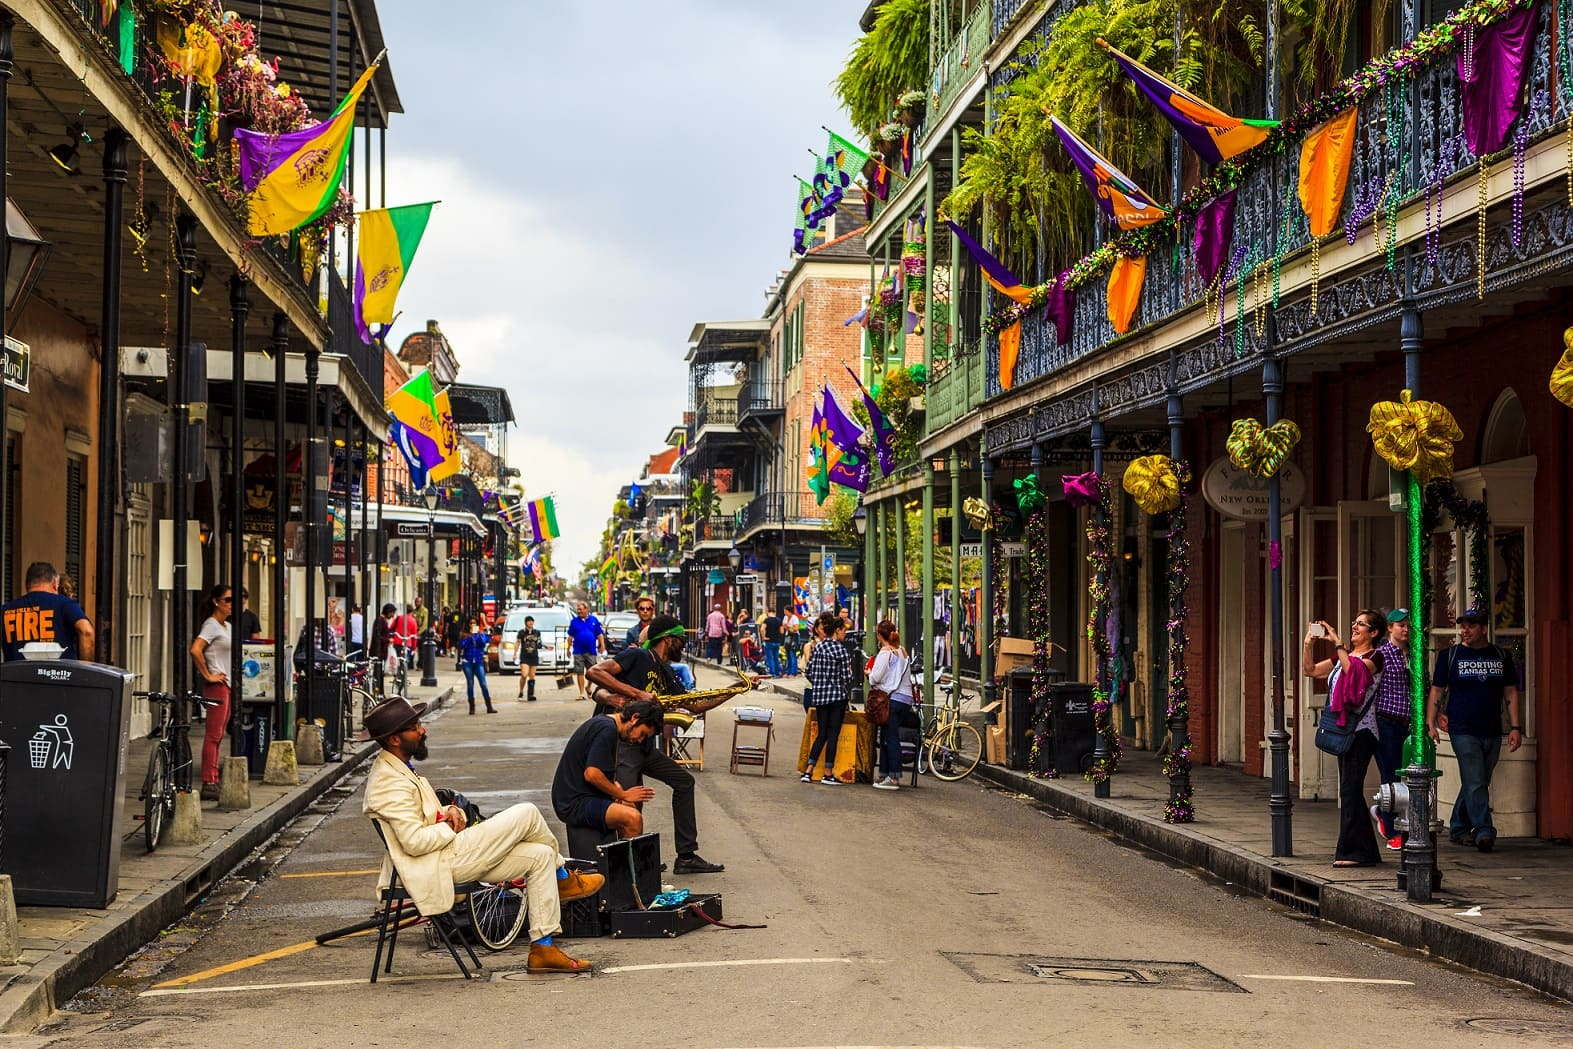
\includegraphics[scale=0.1]{nola.jpg}
            }
            \only<3-4>{
              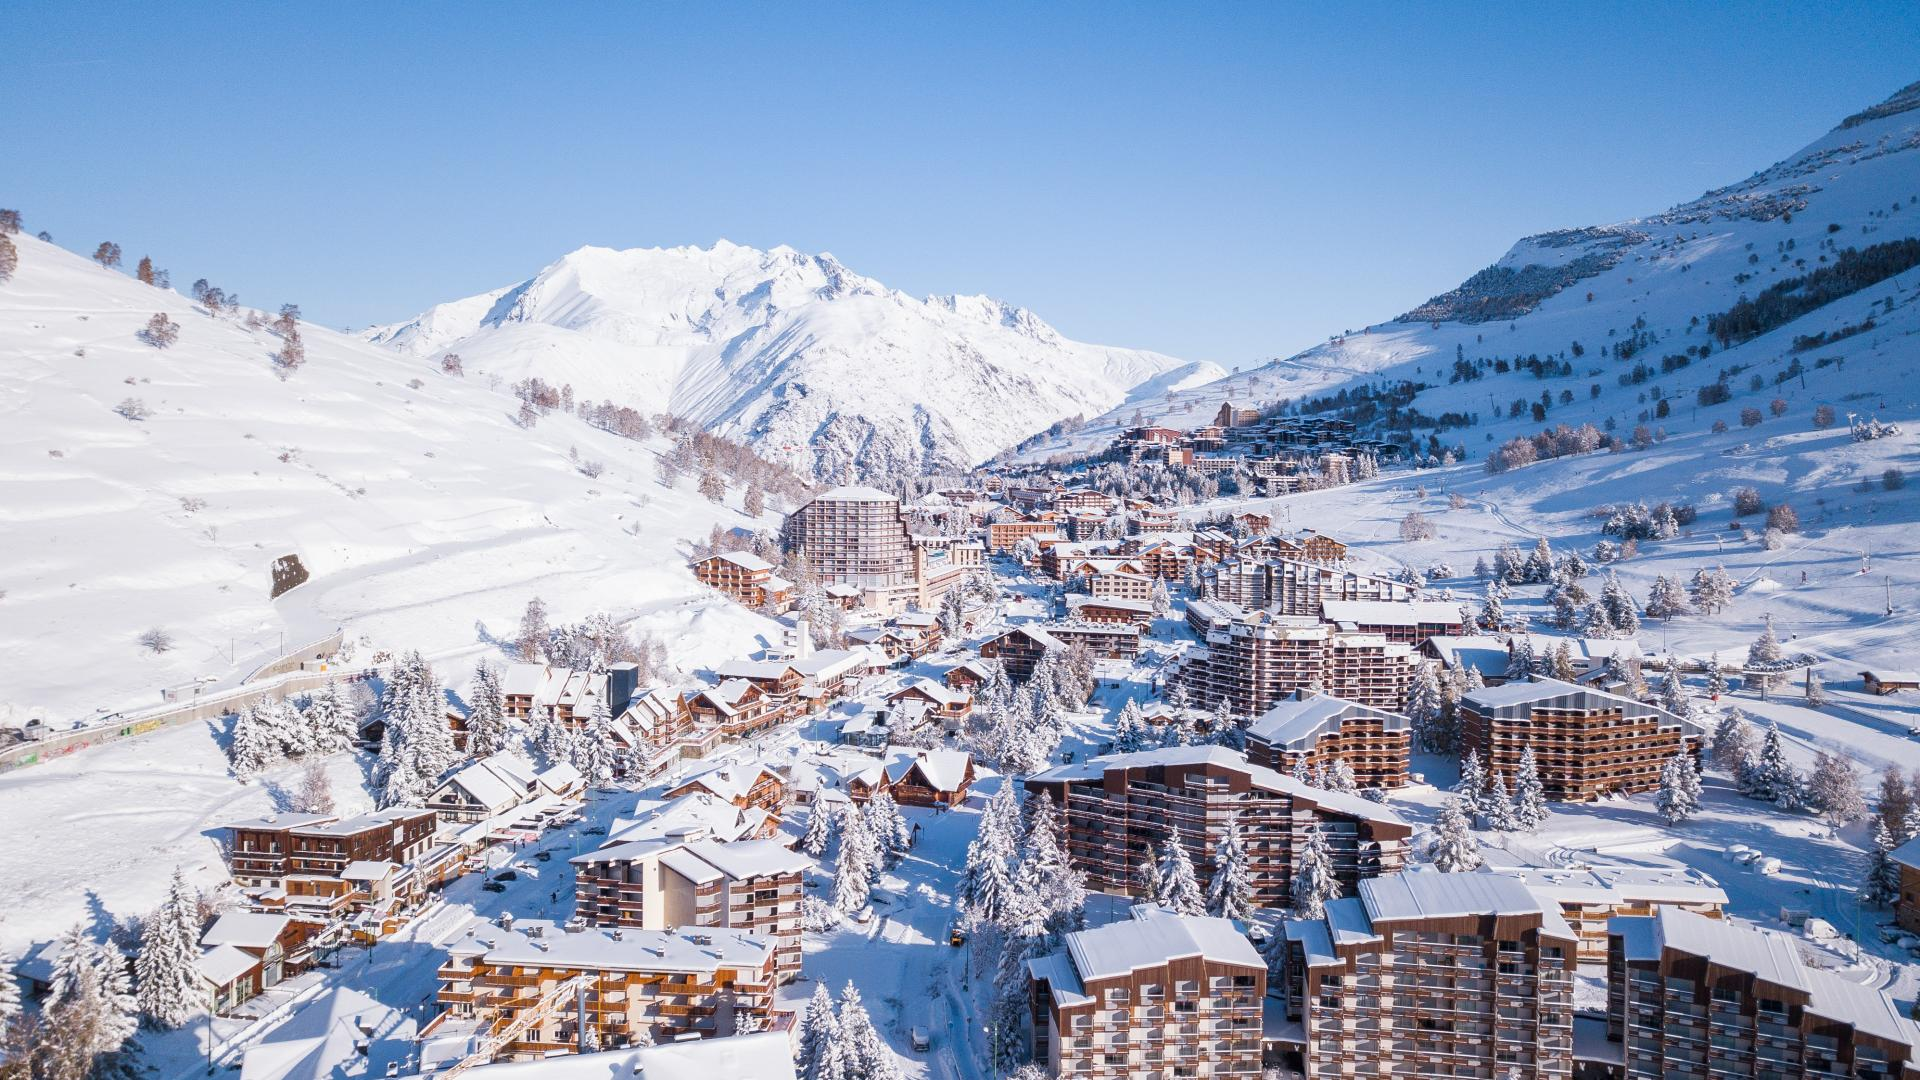
\includegraphics[scale=0.115]{alpes.jpg}
            }
            \only<5-6>{
              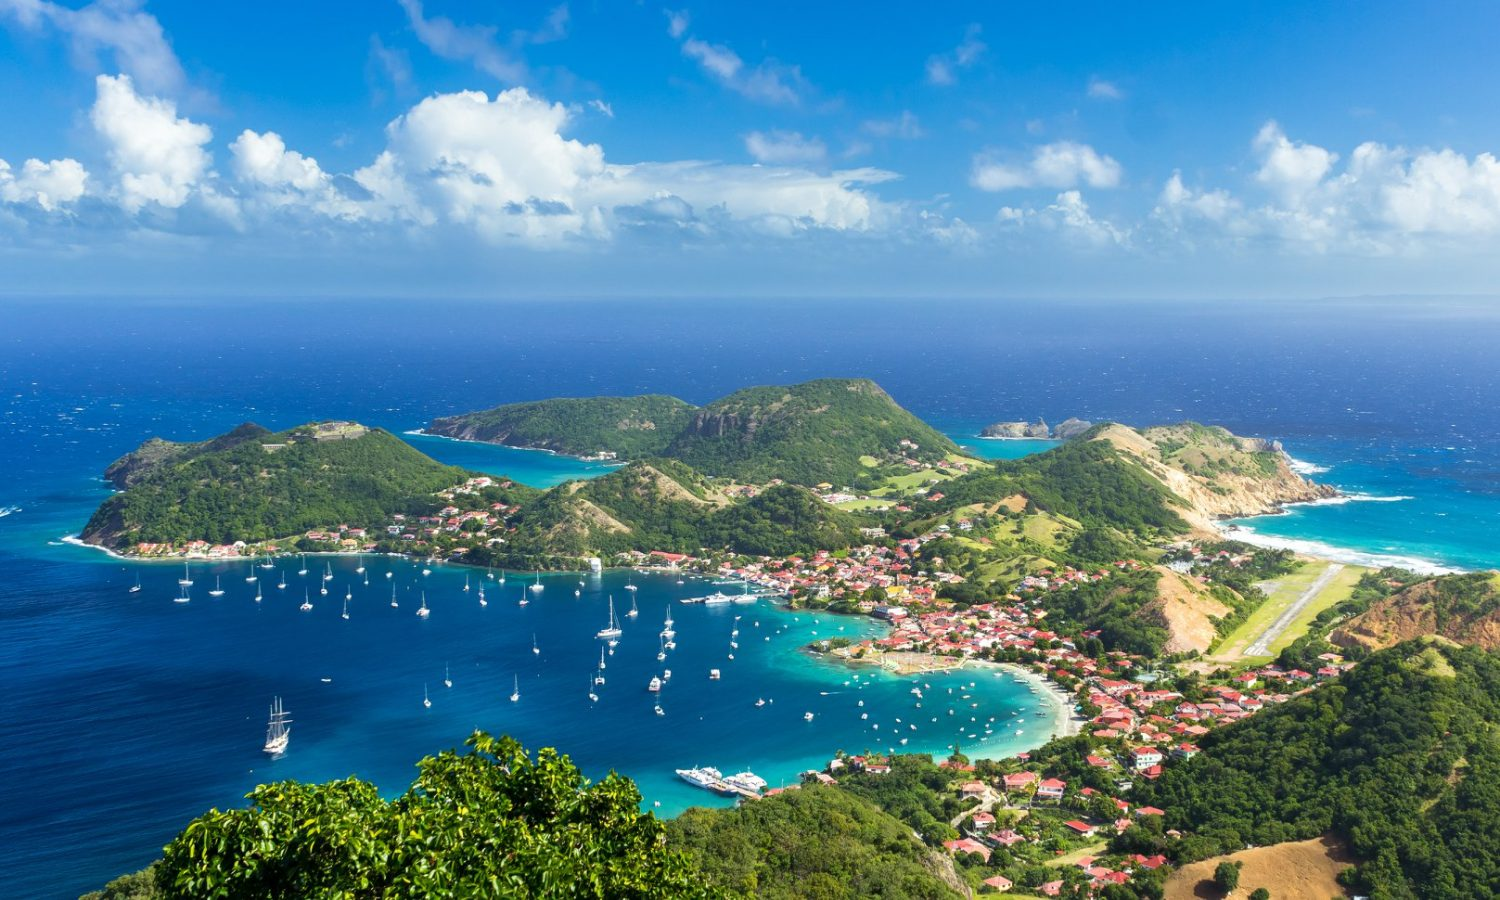
\includegraphics[scale=0.145]{guadeloupe.jpg}
            }
            \only<7-8>{
              \includegraphics[scale=0.125]{mexique_musée.jpg} \\
              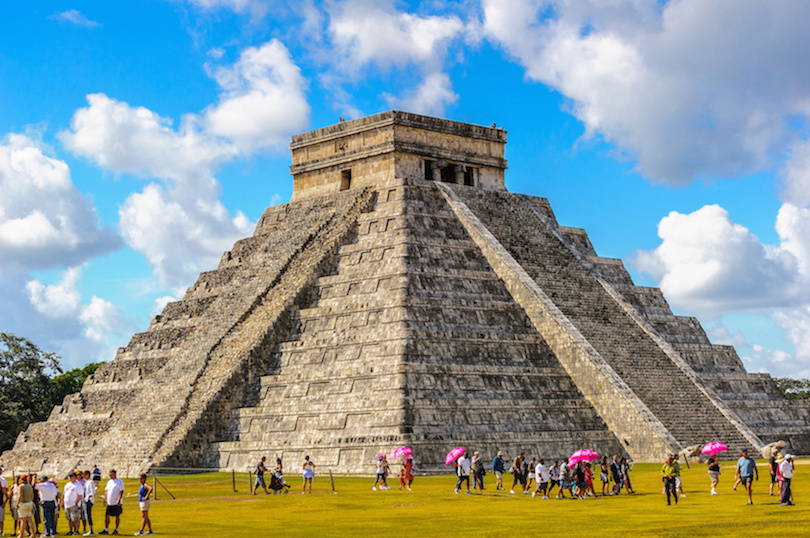
\includegraphics[scale=0.175]{mexique_pyramide.jpg}
            }
          \end{center}
        \end{minipage}
    \end{columns}
  \end{frame}

  \begin{frame}{}
    \begin{center}
      \Large Quiz
    \end{center}
  \end{frame}

  \begin{frame}{Endroits habituels}
    Demande à un/e partenaire s'il ou si elle va aux endroits suivants.
    Il/Elle doit te donner une raison pourquoi.
    \alert{N'oublie pas} d'utiliser le pronom \alert{y} dans tes réponses!
    \begin{columns}[t]
      \column{0.6\textwidth}
        \begin{description}
          \item[] \textbf{Modèle:} \textit{dans des bons restaurants}
          \item[E1:] Tu vas quelquefois dans des bons restaurants?
          \item[E2:] Non, je n'\alert{y} vais jamais.
          \item[E1:] Pourquoi?
          \item[E2:] Parce qu'ils sont très chers, et je n'ai pas assez d'argent pour \alert{y} aller.
        \end{description}
      \column{0.4\textwidth}
        \begin{enumerate}
          \item au théâtre
          \item à des concerts
          \item dans un café
          \item au musée
          \item à la plage
          \item à la montagne
          \item en Europe
          \item dans un pays francophone
        \end{enumerate}
    \end{columns}
  \end{frame}

  \begin{frame}{}
    \begin{center}
      \Large Questions?
    \end{center}
  \end{frame}
\end{document}
